\documentclass[12pt]{article}  

%%%%%%%% PREÁMBULO %%%%%%%%%%%%
\title{Portada reporte practicas}

\usepackage{tikz}
\usetikzlibrary{positioning, arrows.meta}
\usetikzlibrary{shapes.geometric, arrows}
\usetikzlibrary{positioning, arrows.meta}
\usetikzlibrary{positioning, arrows.meta}
\usepackage[spanish]{babel} 
\usepackage[utf8]{inputenc}    
\usepackage{amsmath} 
\usepackage{xcolor}

%\usepackage{amssymb} 
\usepackage{graphicx} 
\usepackage{color} 
\usepackage{subfigure} 
\usepackage{float} 
\usepackage{capt-of} 
\usepackage{sidecap} 
	\sidecaptionvpos{figure}{c} 
\usepackage{caption} 
\usepackage{commath}  

\usepackage{cancel} 
 
\usepackage{anysize} 					
\marginsize{2cm}{2cm}{2cm}{2cm} 

\usepackage{appendix}
\renewcommand{\appendixname}{Apéndices}
\renewcommand{\appendixtocname}{Apéndices}
\renewcommand{\appendixpagename}{Apéndices} 

\usepackage[colorlinks=true,plainpages=true,citecolor=blue,linkcolor=blue]{hyperref}

\usepackage{fancyhdr} 
\pagestyle{fancy}
\fancyhf{}
\fancyhead[L]{\footnotesize UPIITA} 
\fancyhead[R]{\footnotesize IPN}   
\fancyfoot[R]{\footnotesize Programacion Avanzada}  
\fancyfoot[C]{\thepage} 
\fancyfoot[L]{\footnotesize Ing. Mecatrónica}  
\renewcommand{\footrulewidth}{0.4pt}


\usepackage{listings} 
\definecolor{dkgreen}{rgb}{0,0.6,0} 
\definecolor{gray}{rgb}{0.5,0.5,0.5}

\tikzstyle{startstop} = [rectangle, rounded corners, minimum width=3cm, minimum height=1cm,text centered, draw=black, fill=red!30]
\tikzstyle{process} = [rectangle, minimum width=3cm, minimum height=1cm, text centered, draw=black, fill=orange!30]
\tikzstyle{io} = [trapezium, trapezium left angle=70, trapezium right angle=110, minimum width=3cm, minimum height=1cm, text centered, draw=black, fill=blue!30]
\tikzstyle{decision} = [diamond, minimum width=3cm, minimum height=1cm, text centered, draw=black, fill=green!30]
\tikzstyle{arrow} = [thick,->,>=stealth] 

% configuración para el lenguaje que queramos utilizar
\lstnewenvironment{python}[1][]
{
    \lstset{
        language=Python,
        basicstyle=\small\ttfamily,
        keywordstyle=\color{blue}\bfseries,
        commentstyle=\color{green!60!black},
        stringstyle=\color{red},
        showstringspaces=false,
        frame=single,
        numbers=left,
        numberstyle=\tiny,
        numbersep=5pt,
        #1
    }
}
{}
\title{Plantilla portada}

%%%%%%%% TERMINA PREÁMBULO %%%%%%%%%%%%

\begin{document}

%%%%%%%%%%%%%%%%%%%%%%%%%%%%%%%%%% PORTADA %%%%%%%%%%%%%%%%%%%%%%%%%%%%%%%%%%%%%%%%%%%%
																					%%%
\begin{center}																		%%%
\newcommand{\HRule}{\rule{\linewidth}{0.5mm}}									%%%\left
 																					%%%
 																					
\begin{minipage}{0.48\textwidth} \begin{flushleft}

\includegraphics[scale = 0.63]{logo_upiita.png}
\end{flushleft}\end{minipage}
\begin{minipage}{0.48\textwidth} \begin{flushright}

\includegraphics[scale = 0.35]{IPN.jpg}
\end{flushright}\end{minipage}

													 								%%%
\vspace*{-1.5cm}								%%%
																					%%%	
\textsc{\huge Instituto Polit\'ecnico\\ \vspace{5px} Nacional}\\[1.5cm]	

\textsc{\LARGE Unidad Profesional Interdisciplinaria en Ingenier\'ia y				%%%
Tecnolog\'ias Avanzadas}\\[1.5cm]													%%%

\begin{minipage}{0.9\textwidth} 
\begin{center}																					%%%
\textsc{\LARGE Programación Avanzada 2MV7}
\end{center}
\end{minipage}\\[0.5cm]
%%%
    																				%%%
 			\vspace*{1cm}																		%%%
																					%%%
\HRule \\[0.4cm]																	%%%
{ \huge \bfseries Practica 3}\\[0.4cm]	%%%
 																					%%%
\HRule \\[1.5cm]																	%%%
 																				%%%
																					%%%
\begin{minipage}{0.46\textwidth}													%%%
\begin{flushleft} \large															%%%
\emph{Autor:}\\	
Barrios Mendez Jose Alberto\\
Boleta: 2022640111


%%%
			%\vspace*{2cm}	
            													%%%
										 						%%%
\end{flushleft}																		%%%
\end{minipage}		
																%%%
\begin{minipage}{0.52\textwidth}		
\vspace{-0.6cm}											%%%
\begin{flushright} \large															%%%
\emph{Profesor:} \\																	%%%
Cruz Mora Jose Luis\\
													%%%
\end{flushright}																	%%%
\end{minipage}	
\vspace*{1cm}
%\begin{flushleft}
 	
%\end{flushleft}
%%%
 		\flushleft{\textbf{\Large Ing. Mecatrónica}	}\\																		%%%
\vspace{2cm} 																				
\begin{center}																					
{\large \today}																	%%%
 			\end{center}												  						
\end{center}							 											
																					
\newpage																		
%%%%%%%%%%%%%%%%%%%% TERMINA PORTADA %%%%%%%%%%%%%%%%%%%%%%%%%%%%%%%%

\tableofcontents 

\newpage

\section{Objetivo.}

Desarrollar programas utilizando la herencia y polimorfismo.

\section{Introduccion.} 
Para esta practica continuamos con la programacion orienteda a objetos en python, en el desarrollo de esta practica tendremos la implementacion de una tienda de mascotas, la cual esta dividida en categorias, donde aplicaremos la herencia, que es un pilar fundamental de la programacion orientada a objetos. Ademas tendremos una seccion donde desarrollaremos la herencia en clases de computadoras,crearemos objetos distintos como lo son telefonos, pc, laptops.\\
Estas practicas se desarrollan con el fin de implementar la herencia asi que lo trataremos mas a detalle a continuacion:\\


\section{Desarrollo.}
\subsection{Computadoras.}
Para el desarollo del codigo debemos percatarnos que vamos a tener una herencia desde una clase de tipo Interfaz hacia 4 clases diferentes, las cuales son: Computadora portatil, Computadora de Escritorio, Telefono inteligente, Tablet. Donde a pesar que estas clases son diferentes todas van a heredar los atributos del clase abstracta. En la clase abstracta vamos a tener los atributos de Memoria, Procesador, Almacenamiento, GPU. ademas de tener declarados sus respectivos getters y setters de forma abstracta, es decir, solo se declara para que el programa este al tanto de los metodos que las clases que heredan de la clase computadora deveran implementarlos al crear una instancia, o por decirlo de otra forma, obligarlos a declarar todos sus atributos cada que se crea un objeto. vamos a analizar el codigo.Primero creamos la clase Computadora, declaramos el iniciador con los atrivutos antes mencionados, para aplicar el encapsulamiento nosotros declaramos los atrivutos como privados, aunque en python estos no aplican del todo, es bueno considerarlos para llevar acabo una buena practica de programacion. Cabe recordar que en python para crear los atributos privados es de la forma .
\_\_variable
\begin{figure}[H]
		\begin{center}
 			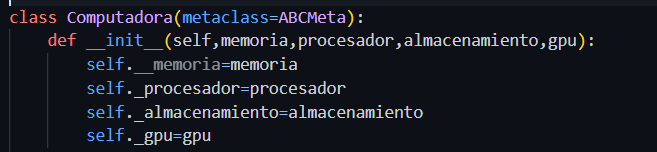
\includegraphics[width = .8\textwidth]{01.png}
 			\captionof{figure}{\label{fig:IPN}Creacion de la clase Computadora con sus respectivos atrivutos privados} 
 			
		\end{center} 
\end{figure}

Posteriormente, considerando que es una clase abstracta, es importante que todos los getters que declaremos dentro de esta clase tambien deben ser abstractos, esto con la finalidad de obligar al usuario a declarar los atributos al iniciar esta clase, ademas de que no se podran crear las instancias directamente de esta clase. \\
Para crear los getters abstractos soccorremos al decoraror @property
y del decorador @abstractmethod. Observese en la figura 2.
\begin{figure}[H]
		\begin{center}
 			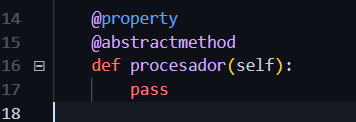
\includegraphics[width = .6\textwidth]{02.png}
 			\captionof{figure}{\label{fig:IPN}Creacion de la clase Computadora con sus respectivos atrivutos privados} 
 			
		\end{center} 
\end{figure}

Para satisfacer los requerimientos solicitados en la practica, se crean todos los getters de cada atrivuto, de la misma forma como defininos el getter para el atrivuto procesador, ilustrado en la imagen, recordando nuevamente que estos getters no se implementan en la clase abstracta, es la clase a la que heredamos quien se va a encargar de sobreescribir el metodo para que indique la forma de este metodo.\\
Posteriormente vamos a crear las subclases que heredaran de la clase Computadora,es importante mencionar que para cada subclase es necesario sobreescribir todos los getters y setters, ya que como estas van a  crear instancias u objetos, no puden estar definidas de la forma abstracta, cada subclase tendra un atrivuto adicional, ademas de un metodo respectivamente para el atributo, las subclases son.\\
\begin{itemize}

\item Computadora portatil: Para esta subclase fue necesario agregrar un atrivuto protegido llamado tamaño, el cual indica el tamaño de esta misma, los getters y setters quedarian de la forma:
\begin{figure}[H]
		\begin{center}
 			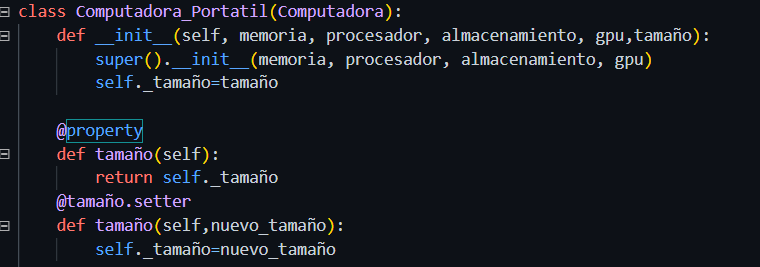
\includegraphics[width = .6\textwidth]{03.png}
 			\captionof{figure}{\label{fig:IPN}Subclase con el atributo y getters and setters de tamaño}
 			 	
		\end{center} 
\end{figure}
Es importente mencionar que cada subclase sobreescribe cada setter y getter, pero para fines practicos solo mostraremos los que son diferentes entre cada clase

\item Computadora Escritorio: Para esta clase solo vamos a definir el atributo y el metodo con sus respectivos getters and setter para el tipo de bocinas que contiene la computadora de escritorio, veamoslo 
\begin{figure}[H]
		\begin{center}
 			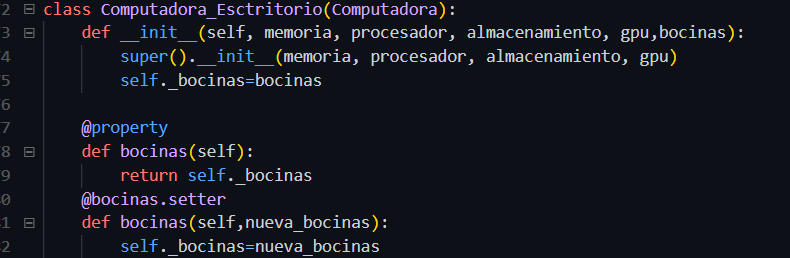
\includegraphics[width = .6\textwidth]{04.png}
 			\captionof{figure}{\label{fig:IPN}Subclase con el atributo y getters and setters de bocinas}
 			 	
		\end{center} 
\end{figure}

\item Telefono Inteligente: Para esta subclase, lo que va a hacerla diferente va a ser el atrivuto camara, que describiria en un principio la capacidad de esta
\begin{figure}[H]
		\begin{center}
 			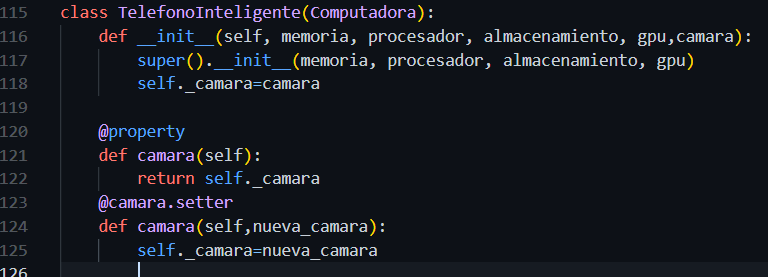
\includegraphics[width = .6\textwidth]{05.png}
 			\captionof{figure}{\label{fig:IPN}Subclase con el atributo y getters and setters de camara}
 			 	
		\end{center} 
\end{figure}

\item Tablet: Para esta subclase la diferencia es que tendremos el atrivuto pantalla
\begin{figure}[H]
		\begin{center}
 			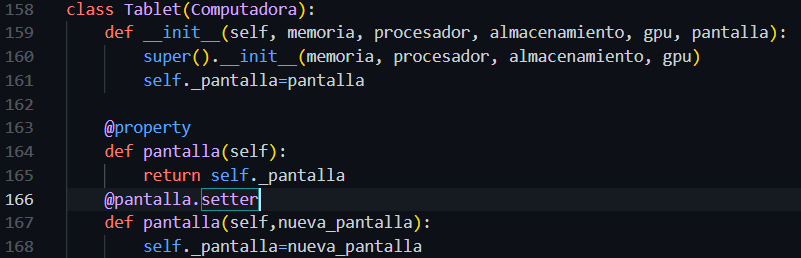
\includegraphics[width = .6\textwidth]{06.png}
 			\captionof{figure}{\label{fig:IPN}Subclase con el atributo y getters and setters de pantalla}
 			 	
		\end{center} 
\end{figure}

\end{itemize}

Una vez que hemos definido cada subclase, queda lo mas importante, que es crear los objetos, como sugerencia o instruccion de la practica, nos pide crear al menos 3 objetos por cada subclase, por lo que tendriamos un total de 12 objetos, como estamos utilizando una interfaz o clase abstracta, es necesario que al crea cada objeto, inicializemos todos sus atributos, con la ayuda de los setters, podemos modificar cada atrivuto posterior a su creacion. veamos en la imagen la creacion de  los objetos 
\begin{figure}[H]
		\begin{center}
 			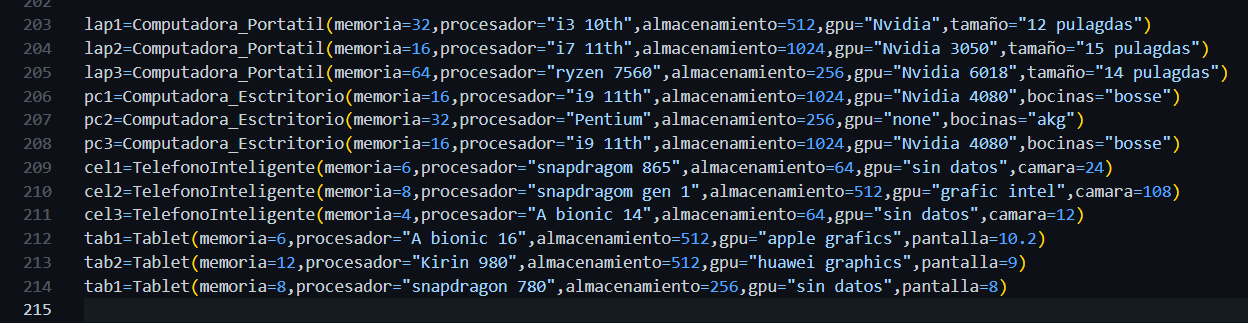
\includegraphics[width = .8\textwidth]{07.png}
 			\captionof{figure}{\label{fig:IPN}Creacion de los objetos iniciando sus atributos}
 			 	
		\end{center} 
\end{figure}

\subsection{Mascotas.}
El objetivo de esta practica es llevar a cabo la herencia en pyhton, la practica nos pide crear varias clases abstractas, comenzando con la clase Mascota, la cual contiene los atributos de: nombre,edad,dueño,tipo. Asi como sus respectivos getters, es importente mencionar que el diagrama de clases nos pide adicionalmente 2 metodos aparte, los cuales son el metodo habla y el metodo toString() que para fines practicos e definido como un metodo str, este metodo se usara para imprimir los datos mas adelante
los metodos adicionales son creados de la siguiente forma
\begin{figure}[H]
		\begin{center}
 			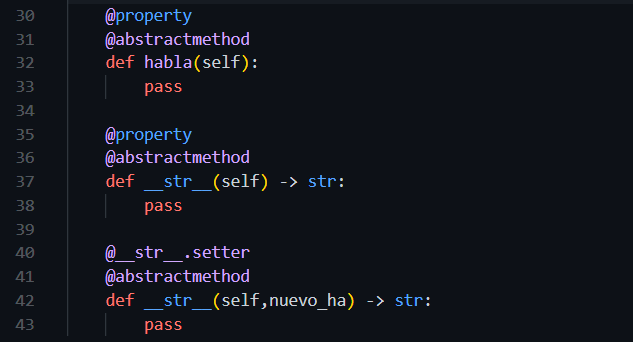
\includegraphics[width = .9\textwidth]{09.png}
 			\captionof{figure}{\label{fig:IPN}Creacion de los metodos abstractos habla y str}
 			 	
		\end{center} 
\end{figure}

Posteriormente esta clase abstracta sera la plantilla para crear otras 2 clases abstractas, que seran las clases Domestica y Exotica.\\
Domestica: Para esta clase se  nos pide agregar un nuevo atributo que es el de nivel de ternura, con sus respectivo set y get, ya que este valor si puede ser modificado.
\begin{figure}[H]
		\begin{center}
 			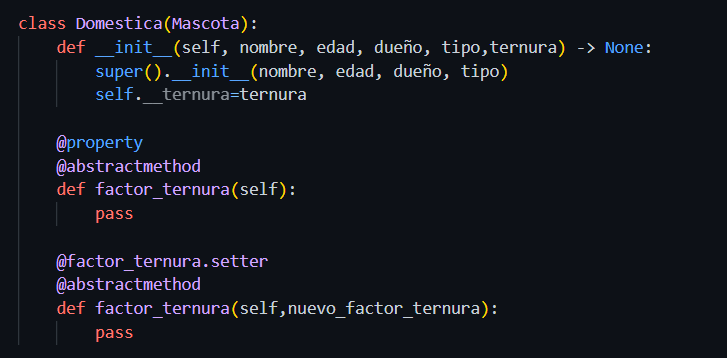
\includegraphics[width = .9\textwidth]{10.png}
 			\captionof{figure}{\label{fig:IPN}Creacion de la clase abstracta Domestica con el metodo ternura}
 			 	
		\end{center} 
\end{figure}

Por su contraparte tenemos la clase abstracta, a comparacion con la clase Domestica este va a tener el metodo Peligro.
\begin{figure}[H]
		\begin{center}
 			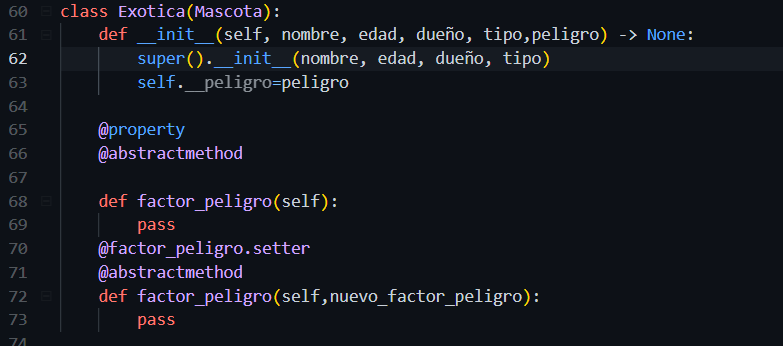
\includegraphics[width = .9\textwidth]{11.png}
 			\captionof{figure}{\label{fig:IPN}Creacion de la clase abstracta Exotica con el metodo peligro}
 			
 			 	
		\end{center} 
\end{figure}

De la clase Domestica se generan 2 subclases que son Perro y Gato, para estas clases se deben reescribir los metodos, ya que a partir de esta clase si se generan objetos. Para ejemplificar mostraremos los metodos habla y str de la clase Gato
\begin{figure}[H]
		\begin{center}
 			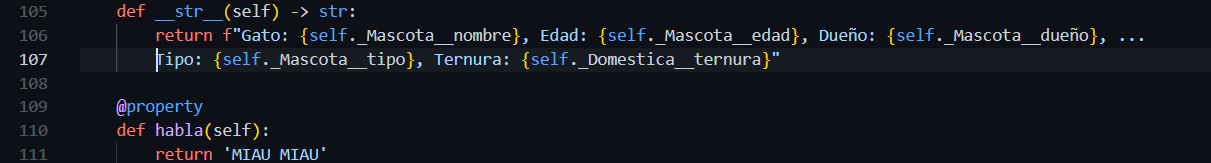
\includegraphics[width = .9\textwidth]{12.png}
 			\captionof{figure}{\label{fig:IPN}sobre escritura de los metodos habla y str de la clase Gato}
 			
 			 	
		\end{center} 
\end{figure}

Para la herencia de la clase Exotica vamos a encotrar que este genera clases con el atributo peligro, las subclases que heredan esto son: vivora,tigre,dinosaurios. Veamos un ejemplo de la sobre escritura de los metodos habla y str de un dinosaurio
\begin{figure}[H]
		\begin{center}
 			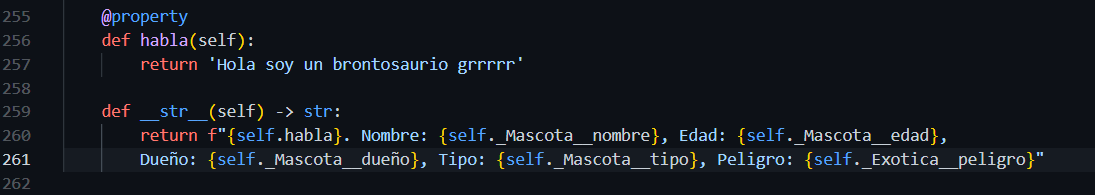
\includegraphics[width = .9\textwidth]{13.png}
 			\captionof{figure}{\label{fig:IPN}sobre escritura de los metodos habla y str de la clase Brontosaurio}
 			
 			 	
		\end{center} 
\end{figure}
Una vez que hemos creado todas las clases con ayuda de la herencia, dejamos este archivo para exportarlo como un modulo posteriormente, en un nuevo programa creamos la estructura para el menu dentro al momento de ejecutarlo y este sea de una forma mas legible y con ayuda de funciones para poder validar los datos de entrada, nos es posible crear los objetos, aunado a un ciclo while donde se encuentra la parte principal del codigo: 
\begin{figure}[H]
		\begin{center}
 			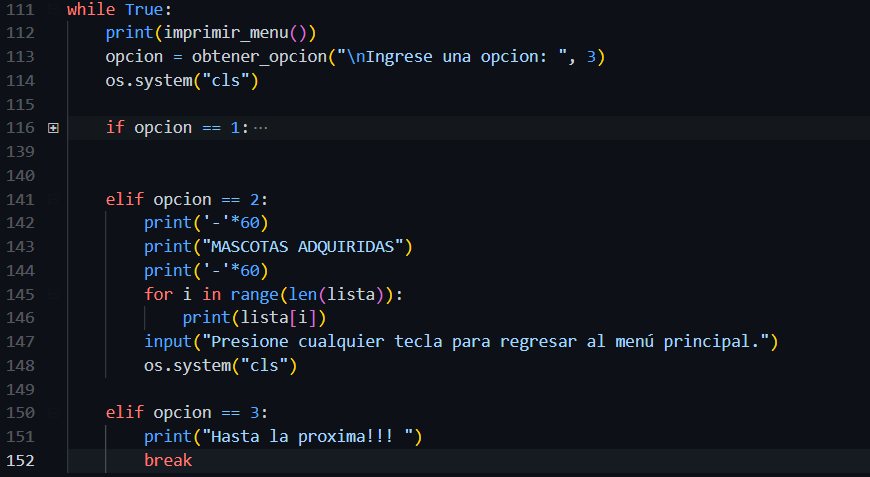
\includegraphics[width = .9\textwidth]{14.png}
 			\captionof{figure}{\label{fig:IPN}codigo para añadir mascotas como desee el usuario}
 			
 			 	
		\end{center} 
\end{figure}
en el codigo se puede observar que llamanos la funcion menu para mostrarlo en pantalla, preguntamos sobre la opcion que el usuario desea hacer, en caso de ser 1, se desplega otro menu para mostrar las mascotas, en el caso 2, se muestran las mascotas adquiridas, en la opcion 3 es para salir del programa

\section{Resultados}
\subsection{Computadora}
Al momento de ejecutar el codigo nos va a mostrar todos los objetos con sus caracteristicas, tal como se muestra en la siguiente figura.
 \begin{figure}[H]
		\begin{center}
 			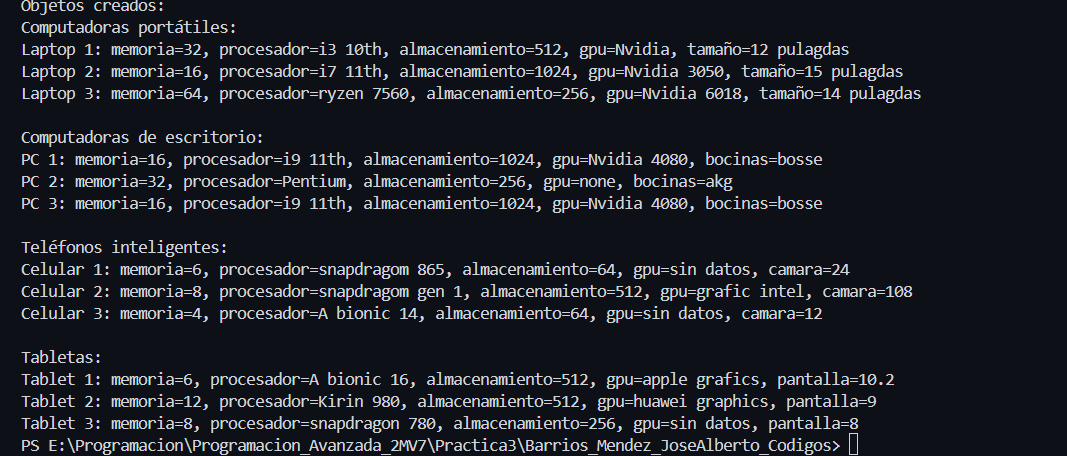
\includegraphics[width = .9\textwidth]{08.png}
 			\captionof{figure}{\label{fig:IPN}Ejecucion del programa numero 1}
 			 	
		\end{center} 
\end{figure}
Es importante mencionar que al usar los setters es posible modificar los valores de cada atributo, esto se puede llevar a cabo de la siguiente forma  \textbf{lap1.memoria=67}, lo cual lo convierte en una forma mas sencilla de poder sobreescribir lo que en un principio se definio al momento de crear el objeto

\subsection{Mascotas}
Al ejecutar el programa nos arroja lo siguiente
\begin{figure}[H]
		\begin{center}
 			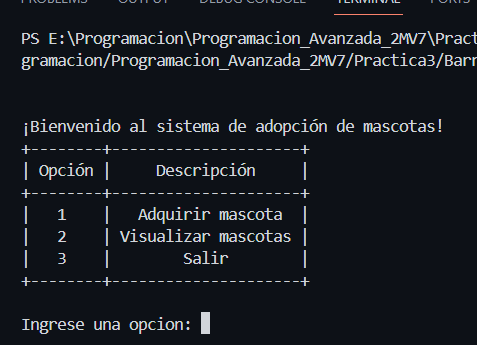
\includegraphics[width = .7\textwidth]{15.png}
 			\captionof{figure}{\label{fig:IPN}Resultado al ejecutar el programa}
 			
 			 	
		\end{center} 
\end{figure}
vamos a empezar con añadir una mascota, que es la opcion 1:
\begin{figure}[H]
		\begin{center}
 			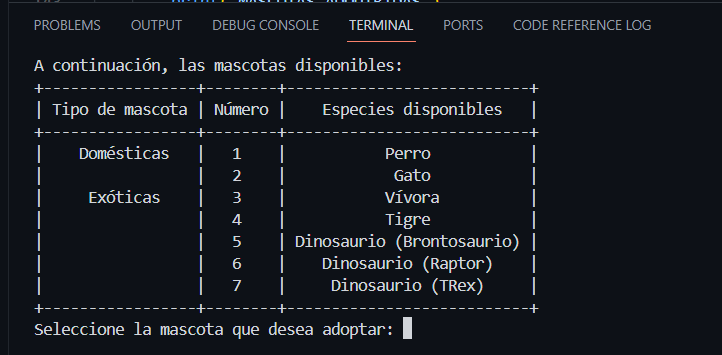
\includegraphics[width = .7\textwidth]{16.png}
 			\captionof{figure}{\label{fig:IPN}Segundo menu para elegir una mascota}
 			
 			 	
		\end{center} 
\end{figure}

Al seleccionar una opcion por ejemplo Gato (opcion 4) el programa procede a solicitar los datos:
\begin{figure}[H]
		\begin{center}
 			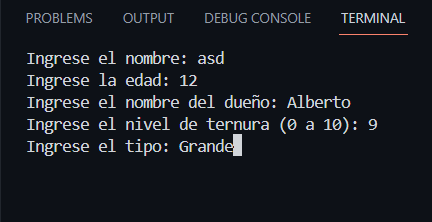
\includegraphics[width = .7\textwidth]{17.png}
 			\captionof{figure}{\label{fig:IPN}Ingreso de los datos de la mascota seleccionada}
 			
 			 	
		\end{center} 
\end{figure}

Al terminar de introducir los datos, nos arroja lo siguiente:
\begin{figure}[H]
		\begin{center}
 			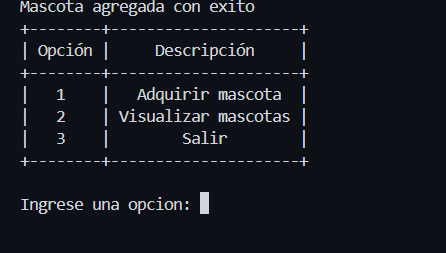
\includegraphics[width = .7\textwidth]{18.png}
 			\captionof{figure}{\label{fig:IPN}Mascota añadida y vuelta al menu}
 			
 			
 			 	
		\end{center} 
\end{figure}

Para mostrar las mascotas adquiridas es suficiente con seleccionar la opcion numero 2:
\begin{figure}[H]
		\begin{center}
 			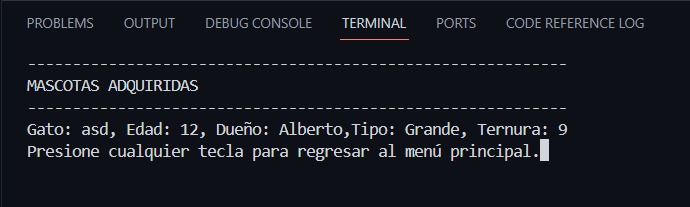
\includegraphics[width = .7\textwidth]{19.png}
 			\captionof{figure}{\label{fig:IPN}Visualizacion de las mascotas adquiridas}
 			
 			 	
		\end{center} 
\end{figure}

\section{Conclusiones.}
Al realizar esta practica, de forma independiente a lo extensa que resulto, 
aunque la programación orientada a objetos puede no siempre conducir a una reducción directa en la cantidad de líneas de código escritas, sus beneficios en términos de mantenimiento, reutilización, flexibilidad y comprensión del código son invaluables. Al adoptar los principios de la programacion orientada a objetos y aplicarlos de manera efectiva en nuestros proyectos, podemos construir sistemas más robustos, flexibles y fáciles de mantener, lo que finalmente conduce a un desarrollo de software más eficiente y exitoso.

%%%%%%% Bibliografía %%%%%%%%    

%\appendix  
%\clearpage % o \cleardoublepage
%\addappheadtotoc 
%\appendixpage

%\section{Anexos 1.}




%\section{Anexos 2.}


 

\end{document}